\chapter{Simulation von Streubildern}
Das Problem der Berechnung synthetischer Streubilder besitzt verschiedene Lösungsansätze..
\section{Mie Streuung}
Die Mie-Theorie bietet eine analytische Lösung der Streuung an einer Kugel  in Form einer unendlichen Reihe basierend auf einer Lösung der Grenzbedingungen für elektromagnetische Wellen \cite{bohren2008}. Die unendliche reihe lässt sich näherungsweise numerisch berechenen (Details siehe Anhang XX). Eine vektorisierte Version dieser Berechnung liegt in der auf Mätzler \cite{maetzler2002} basierenden Matlab Funktionen \texttt{simulation/mie.m} für winkelabhängige Radialprofile sowie \texttt{simulation/mie\_scatter.m} für Streubilder vor und dient der Verifizierung der Simulationsverfahren.

\section{Projektions- und Rayleigh-Gans-Näherung}
	
	Um dreidimensionalen Streuobjekte durch zweidimensionale Blenden zu nähern, lässt sich die Projektion ihrer Dichteverteilung auf eine Ebene direkt hinter ihnen betrachten. In Näherung verhält sich eine elektromagnetische Welle nach Durchlaufen des Objektes gleich wie nach Durchlaufen einer Blende mit dieser durch Projektion gewonnenen Absorption und Refraktion, sodass in Fraunhofer-Fernfeldnäherung das durch Streubild die Fouriertransformierte der Projektion genähert werden kann.
	
	Für eine kreisförmige Blende exisistiert eine analytische Darstellung der Fouriertransformation in Form der sogenannten Airy-Scheibe und das Streubild eines Objektes mit kreisförmiger Projektion lässt sich somit mittels der Besselfunktion 1. Ordnung $J_n$ als
	\begin{equation}
	I(\theta) \propto \left ( \frac{2 J_1(kr \sin \theta)}{kr \sin \theta} \right )^2 
	\end{equation}
	nähern\cite[S. 396]{born1980}. Für nicht kreisförmige Projektionen der Dichte lässt sich die Fouriertransformation diskret numerisch auswerten.
	Eine weitere gebräuchliche Näherung für kugelförmige Objekte ist die Rayleigh-Gans Näherung (gültig für kleine Radien und Brechzahlen nahe Vakuum). In dieser nimmt die Intensität die Form
	\begin{equation}
	    I(\theta)\propto\left ( \frac{j_1(2kr\sin(\theta/2))}{2kr\sin(\theta/2)} \right )^2 
	\end{equation}
	mit der sphärischen Besselfunktion $j_n$ an \cite[S. 163]{bohren2008}. 


\section{Multislice Fourier Transformation}
	Nach XX gilt in der ersten Bornschen Näherung für die Amplitude der gestreuten Welle
	\begin{equation}
		\phi\propto\int \delta\eta(\vec{r}) e^{-i\vec{q}\cdot \vec{r}} \dif \vec{r}
	\end{equation}
    Wird das Skalarprodukt $\vec{q}\cdot \vec{r}=xq_x+yq_yzq_z$ ausgeschrieben und die Integration über $x$ und $y$ als zweidimensionale Fouriertransformation interpretiert
	\begin{equation}
	\phi\propto\int \mathscr{F}\left[\delta\eta\right](q_x,q_y,z) e^{-zq_z} \dif z \, ,
	\end{equation}

	so lässt sich das Integral in z-Richtung als Summe interpretieren sofern sich $q_z$ als $q_z=q_\parallel(q_\perp)$ ausdrücken lässt.
	
	Aufgrund der Impulserhaltung muss $k_{ein}^2=k_{aus}^2=k^2$ gelten. Nach Abbildung XXX ist
	\begin{align}
	k^2=(k-q_\parallel)^2+q_{\perp}^2
	\Leftrightarrow q_\parallel=k-\sqrt{k^2-q_\perp^2}
	\end{align}
	Somit
	\begin{equation}
	\phi\approx\sum_n{\mathscr{F}\left[\rho_z\right] e^{-in\delta_z\left(k-\sqrt{k^2-q_\perp^2}\right) }}
	\end{equation}

	\begin{figure}
		\centering
		
\includegraphics[width=0.5\textwidth]{images/msft.eps}
		\caption[Vektoren bei MSFT]{Skizze zur Bezeichnung der Vektoren. $k_{ein}$ und $k_{aus}$ bezeichnen den Wellenvektor der einfallenden bzw. ausfallenden Welle mit dem dazwischenliegenden Winkel $\theta$. $q$ bezeichnet den Streuvektor mit einer zu $k_{ein}$ parallelen ($q_{||}$) und einer senkrechten ($q_\perp$) Komponente.. }
		\label{fig:msft}
	\end{figure} 

	Formel XXX beschreibt einen Algorithmus um das Streubild eines dreidimensionalen Objektes im Fernfeld in der 1. Bornschen Näherung zu berechnen. Diese Methode wird als Multislice Fourier Transformation (MSFT) bezeichnet \cite{barke2015}. Bei dieser wird Mehrfachstreuung ignoriert. Durch nachträgliches Einführen eines zusätzlichen Faktors XXX der die Absorption und Phasenänderung der Welle beim Durchlaufen des Objektes beschreibt, lässt eine grobe Näherung für Absorptionseffekte einzuführen. Eine Implementation des MSFT-Algorithmus liegt in \texttt{simulation/msft.m} vor 

\section{Multislice Propagation}
	Ein alternatives Verfahren zur Simulation XX ist in der Literatur als Multislice oder Beam Propagation bekannt \cite{hare1994,cowley1957}. Dieses Verfahren basiert auf ...
	Die Szene, deren Streubild zu berechnen ist, wird in einzelne Schichten zerlegt.
	Die Ausbreitung der in Szene einfallende ebene Welle wird genähert durch eine Vakuumpropagation von Schicht zu Schicht nach Angular Spectrum Propagation
	\begin{equation}
\bar{\phi}\left(z+\Delta z\right)=\bar{\phi}(z)e^{i\Delta z\sqrt{k^2-(q_x+q_y)^2}}
	\end{equation}
	sowie eine Wechselwirkung mit der Materie der Schicht in einer einzelnen Ebene
	\begin{equation}
		\phi(z+\Delta z)=\phi e^{i\delta n \Delta z} \, .
	\end{equation}.
	
	\begin{figure}
		\centering
		
\includegraphics[width=0.75\textwidth]{images/multislice.eps}
		\caption[Prinzip Multislice Propagation]{Prinzip Multislice Propagation: Die Szene wird in einzelne Schichten zerlegt und die Wechselwirkung mit der Materie jeder einzelnen Schicht in auf eine in dieser Schicht liegenden Ebene reduziert. Zwischen diesen Ebenen wird eine Vakuumpropagation angewendet.}
		\label{fig:multislice}
	\end{figure} 
	
	Die Näherung der Vakuumausbreitung durch einen Fresnel-Propagator bringt gegenüber der korrekten Berechnung über die Angular Spectrum Propagation keine numerischen Vorteile. Aus diesem Grund wird im Gegensatz zu \cite{hare1994} auf diese Näherung verzichtet. 
	Bei diesem Verfahren wird die Annahme getroffen, dass  innerhalb einer Schicht die örtliche Verteilung der Materie konstant ist, sowie die durch die Propagation bedingte ... vernachlässigbar ist\cite{hare1994}. Des Weiteren wird bei der wird bei der Wechselwirkung mit der Materie der Winkel vernachlässigt XXX.
	
	Der Algorithmus zur Berechnung der Austrittswelle lautet somit
	\begin{equation}
\Phi(z+\Delta z)=
	\end{equation}
	Ist die Austrittswelle bekannt, so ist die weitere Ausbreitung zum Detektor eine Vakuumpropagation, die sich entweder mittels Angular Spectrum Propagation berechnen lässt, oder sich durch eine einfache Fouriertransformation in Fraunhofer-Näherung bestimmen lässt. Ersteres Verfahren hat den Nachteil, das es bei einer numerischen Implementation im Bereich der Szene die gleiche räumliche Rastergröße wie im Bereich des Detektors erfordert, während bei Anwendung der Fernfeld Näherung xxx
\section{Thibaults Multislice}
Thibault stellt in XX einen eigene Formulierung der Multislice-Simulation auf. Ausgehend von der Wellengleichung XX
lässt sich für die Austrittswelle XXX aufstellen.
\begin{equation}
\tilde{\Phi}(z)=\tilde{G}\ast_z\left[\tilde{\delta\eta}\ast_{q_\perp} \tilde{\Phi}\right]
\end{equation}
\begin{equation}
\tilde{G}=\frac{1}{2\pi}\frac{ik^2}{\sqrt{k^2-q_\perp^2}}e^{iz(\kappa-k)}
\end{equation}
unter der Vernachlässigung von Rückstreuung lässt sich das Faltungsintegral in zwei Integrationsbereiche aufspalten
\begin{equation}
\tilde{\Phi}(z+\Delta z)=
\int_{\Delta z}^{\infty} \tilde{G}(z')\left[\tilde{\delta\eta}\ast_{q_\perp} \tilde{\Phi}\right](z+\Delta z-z')\dif z'
+
\int_{0}^{\Delta z} \tilde{G}(z')\left[\tilde{\delta\eta}\ast_{q_\perp} \tilde{\Phi}\right](z+\Delta z-z')\dif z'
\end{equation}
Für den ersten Summanden gilt

\begin{align*}
&\stackrel{\hphantom{z'\rightarrow z''+\Delta z}}{\hphantom{=}} 
\int_{\Delta z}^{\infty} \tilde{G}(z')\left[\tilde{\delta\eta}\ast_{q_\perp} \tilde{\Phi}\right](z+\Delta z-z')\dif z'\\
&\stackrel{z'\rightarrow z''+\Delta z}{=}
\int_{0}^{\infty} \tilde{G}(z''+\Delta z)\left[\tilde{\delta\eta}\ast_{q_\perp} \tilde{\Phi}\right](z-z'')\dif z''\\
&\stackrel{\hphantom{z'\rightarrow z''+\Delta z}}{=}
e^{i\Delta z(\kappa-k)}\int_{0}^{\infty} \frac{1}{2\pi}\frac{ik^2}{\sqrt{k^2-q^2_\perp}}e^{iz''(\kappa-k)}\left[\tilde{\delta\eta}\ast_{q_\perp} \tilde{\Phi}\right](z-z'')\dif z''\\
&\stackrel{\hphantom{z'\rightarrow z''+\Delta z}}{=}
e^{i\Delta z(\kappa-k)}\tilde{\Phi}(z) \numberthis
\end{align*}
Im zweiten Summanden kann für hinreichend kleine $\Delta z$ das Integral gut durch eine Rieman-Obersumme mit einem einzigen Stützpunkt approximiert werden:
\begin{equation}
\int_{0}^{\Delta z} \tilde{G}(z')\left[\tilde{\delta\eta}\ast_{q_\perp} \tilde{\Phi}\right](z+\Delta z-z')\dif z'
\approx
\Delta z \tilde{G}(\Delta z)\left[\tilde{\delta\eta}\ast_{q_\perp} \tilde{\Phi}\right](z)
\end{equation}
Für den Fehler 
\begin{equation}
\text{Rieman Abschätzung}
\end{equation}
Somit lässt sich in Näherung für die Welle bei $z+\Delta z$
\begin{equation}
\tilde{\Phi}(z+\Delta z)
\approx
e^{i\Delta z(\kappa-k)}
\left[
\tilde{\Phi}(z)+\frac{\Delta z}{2\pi}\frac{ik^2}{\sqrt{k^2-q^2_\perp}}
\right]
\end{equation}
Die numerische Simulation dieser Methode ist in \texttt{simulation/thibault.m} implementiert.


\section{Verifizierung}
Zur Verifizierung der vorgestellten Simulationsalgorithmen und deren numerische Implementierungen eignet sich der Vergleich der berechneten Streubilder hinter Kugeln mit den Ergebnissen aus der Berechnung mittels Mie-Streuung. Der Vergleich wird für verschiedene Brechzahlen und Kugelradien bei einer Wellenlänge von 1\si{nm} durchgeführt.

Da ein realer Detektor nicht die Intensitäten bei präzise definierten Winkelpunkten misst sondern innerhalb eines Areals, ist es zweckmäßig, die simulierte Detektorfläche in quadratische Areale zu unterteilen und die Intensität in jedem dieser Areale als gewichtetes Mittel zwischen in dem Areal liegenden Punkten zu betrachten.
Hierbei werden an den Rändern zwischen zwei Arealen liegende Berechnungspunkte zur je zur Hälfte in beiden Arealen, in der Ecke zwischen vier Arealen liegende Berechnungspunkte je zu einem Viertel in den vier Arealen berücksichtigt.
Besonders bemerkbar ist dieser Bearbeitungsschritt bei Pixeln die genau in den Intensitätsminima liegen: Ohne die gewichtete Mittlung würde der gesamten Fläche zwischen den Pixeln die Intensität des Minimums zugewiesen werden, auch wenn dessen Breite extrem schmal ist, werden zusätzliche Pixel berechnet und anschließend gewichtet gemittelt, ergibt sich eine korrektere Wiedergabe des tatsächlichen Intensitätsverlaufs (\fref{fig:average}).

Anschließend werden die simulierten Streubilder bezüglich Verschiebung und Skalierung auf die Mie-Streubilder normiert. Zur Quantifizierung des Fehlers der simulierten Streubilder wird die relative Abweichung von den Mie-Streubildern betrachtet.

Die relative Abbweichung von Mie ist für einen konkreten Parametersatz exemplarisch dargestellt in \fref{fig:relerror}. Aus den rotationssymmetrischen Streubildern können Radialprofile der Intensität sowie des relativen Fehlers bestimmt werden um einen besseren Überblick zu erhalten. \fref{fig:profil}).
Es ist zu erkennen, dass der relative Fehler in den Datenpunkten, in denen das Mie-Profil ein Minimum hat, aufgrund des steilen Verlaufs scharfe,nur 1-2 Datenpunkte umfassende, Maxima annimmt.
Um eine quantifizierende Größe für die Güte einer Simulation bei einem bestimmten Radius und Stoffeigenschaften zu haben, wird deshalb der Median des relativen Fehlers genutzt. So ist es möglich, für die unterschiedlichen Simulationsalgorithmen Bereiche zu bestimmen, in denen sie ausreichend mit der Mie-Theorie übereinstimmen, um sie als in diesem Bereich valide anzusehen \fref{fig:var}. Es ist zu erkennen dass bei Werten von $\delta$ bzw. $\beta$ in der Größenordnung die XXX bei 1\si{nm} Wellenlänge aufweisen sowohl Multislice Propagation und Thibaults Multislice als auch MSFT valide Ergebnisse liefern - der mediane Fehler überschreitet XXX nicht. Bei größeren Abweichungen der Brechzahl von der Vakuumbrechzahl steigt der mediane Fehler des mittels MSFT berechneten Streubildes deutlich an, insbesondere bei großen Radien. Bei diesen kommt es zu deutlich mehr Mehrfachstreuung in Vorwärtsrichtung, die bei MSFT im Gegensatz zu den beiden anderen Multislice Varianten vollständig ignoriert wird. Der Unterschied zwischen Thibaults Multislice Formulierung und der Multislice Propagation kann zu einem gewissen Anteil durch die verwendete naive Implementierung von Thibaults Algorithmus begründet sein. Hier besteht weiteres Optimierungspotential bezüglich der numerischen Genauigkeit und dem Einfluss von Rundungsfehlern.


\begin{figure}
	\centering
	
\includegraphics[width=0.9\textwidth]{images/average.eps}
	\caption[Gewichteter Mittelwert]{Die Verwendung eines gewichteten Mittelwertes zum Binning des Streubildes: Um die Intensität im links rot umrandeten Bereich zu bestimmen, wird die Intensität an den Schwarzen Punkten berechnet und ein gewichteter Mittelwert gebildet, indem die Intensität der vier Randwerte zur Hälfte, die der vier Eckpixel zu einem Viertel in dem umrandeten Bereich mitberücksichtigt werden. Der Effekt gegenüber einer Berchnung nur in den Zentren der Pixel zeigt sich rechts: Wird die Intensität bei einem schwarz dargestellten wahren Intensitätsverlauf nur an den roten Punkten bestimmt, dominiert das Minimum den Intensitätsverlauf. Eine geringere Abweichung ergibt sich bei dem gewichteten Mittelwert (blau).}
	\label{fig:average}
\end{figure} 

\begin{figure}
		\centering
		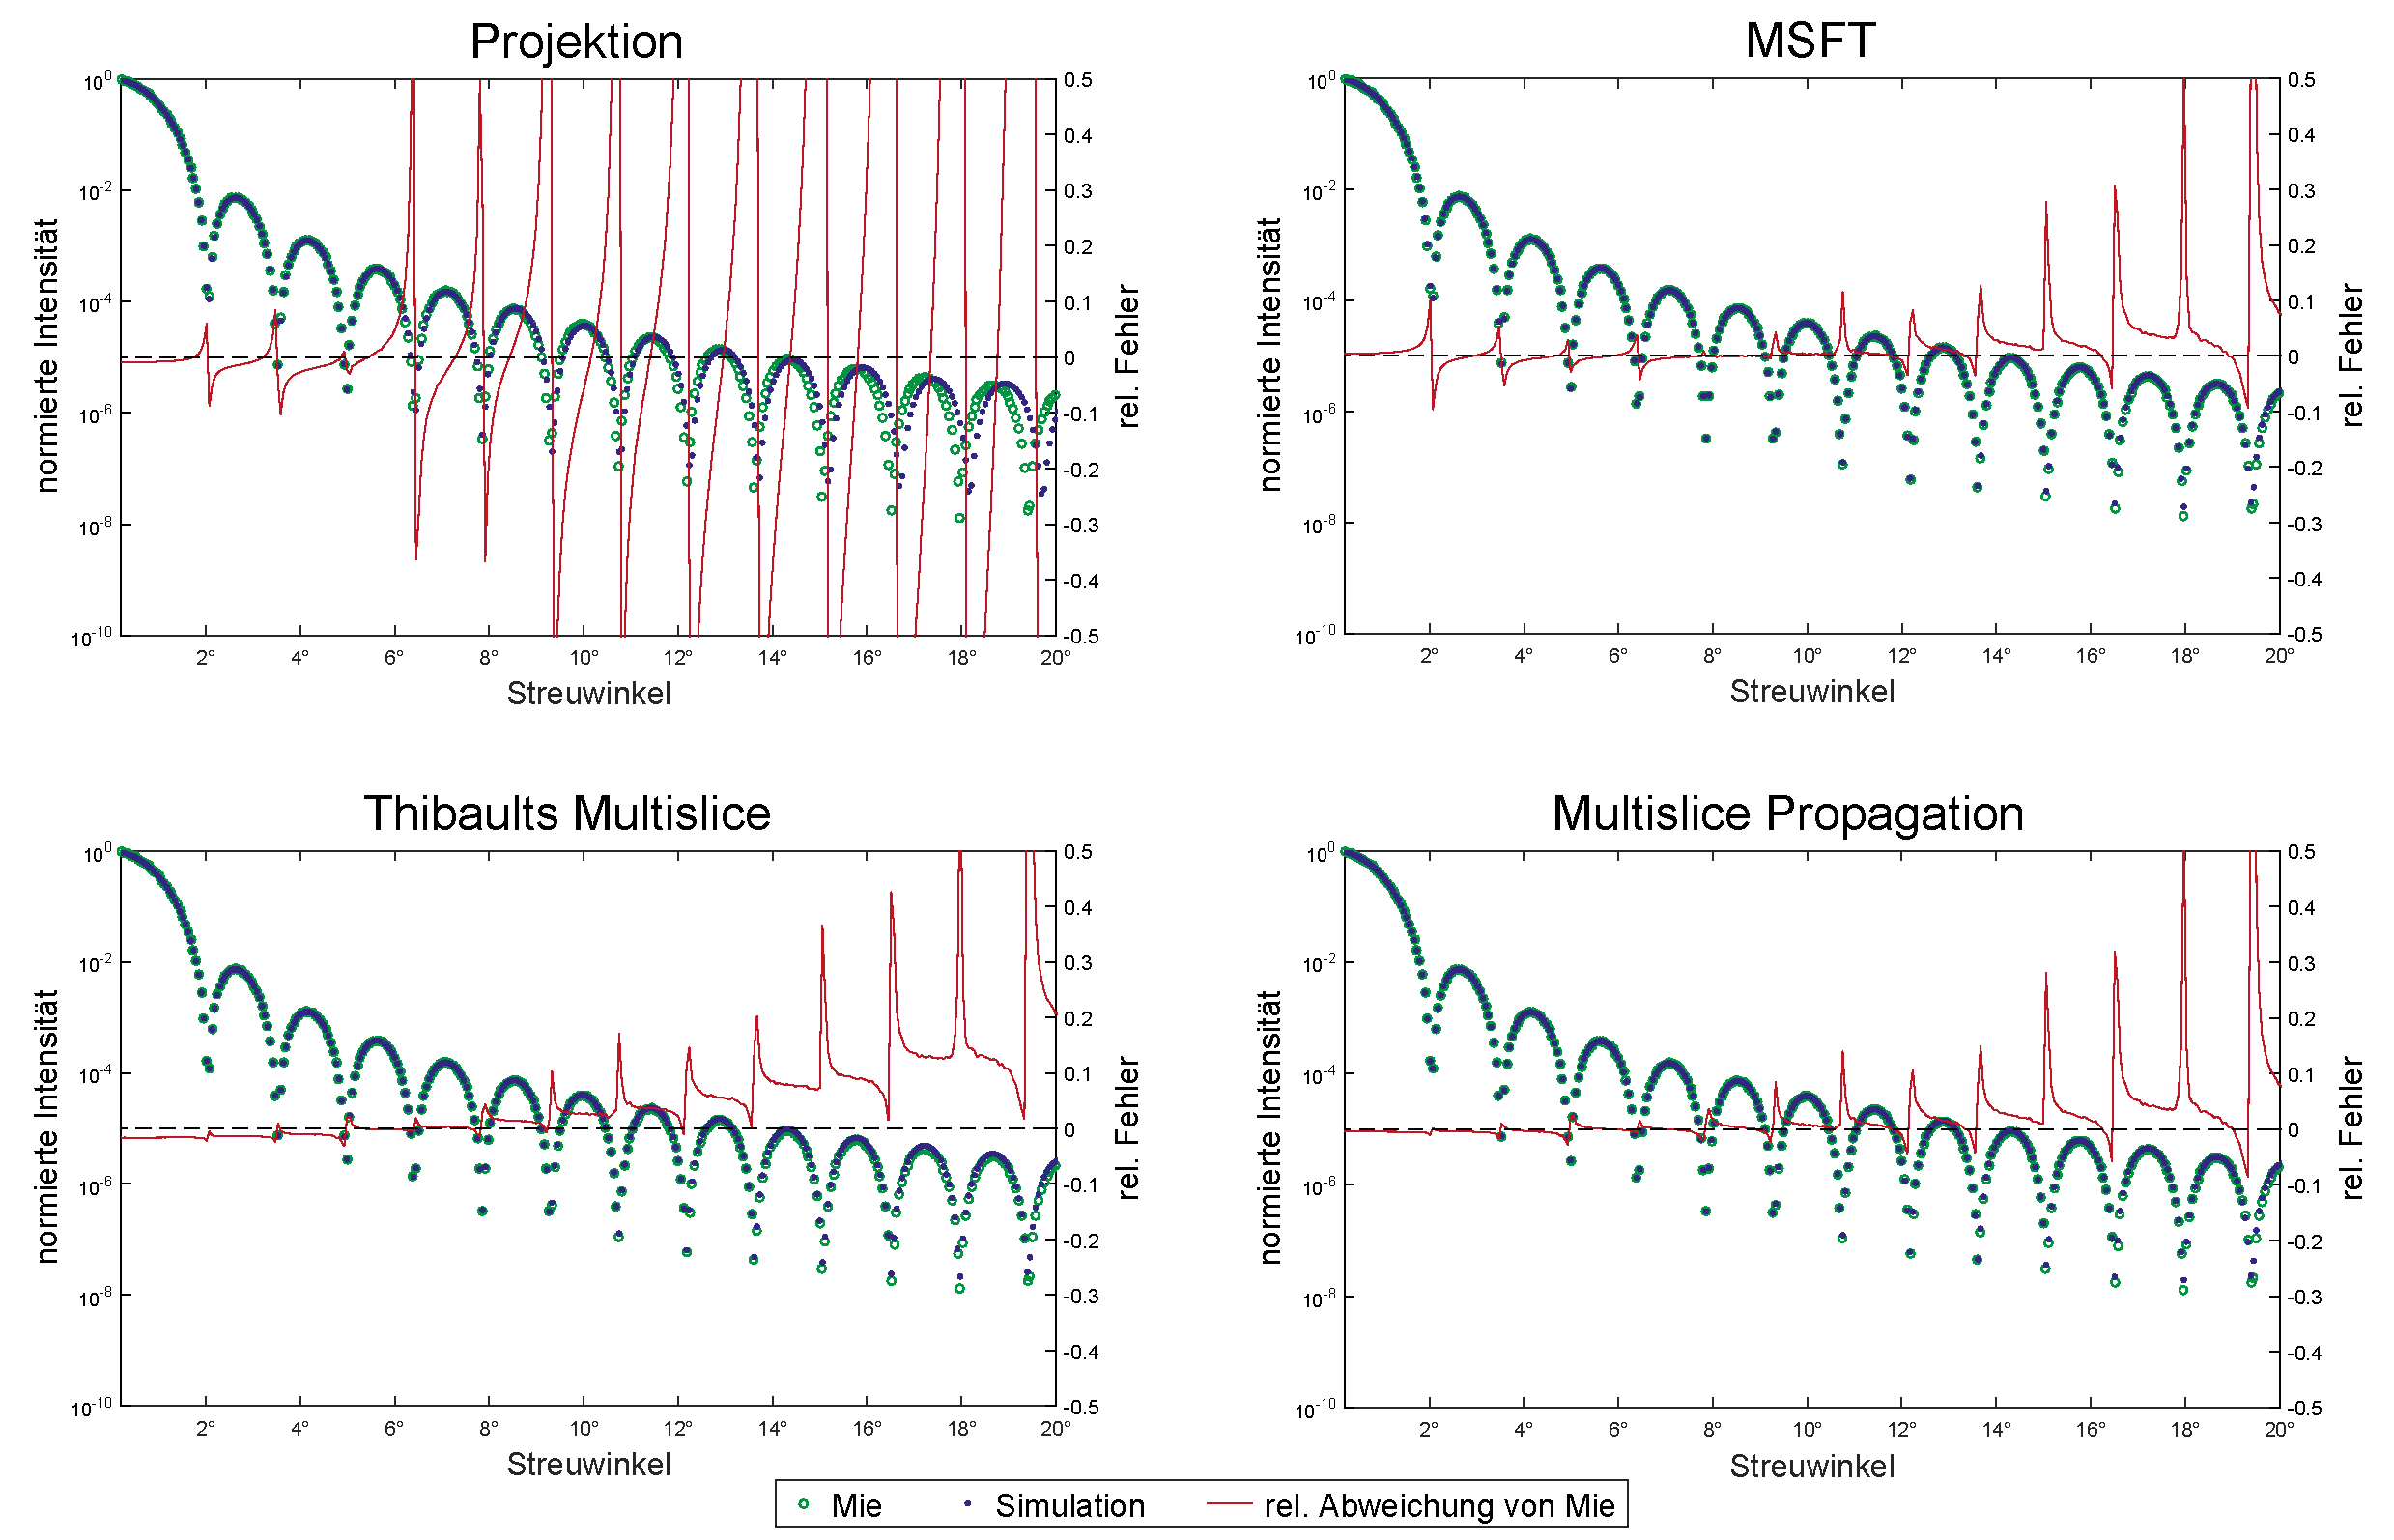
\includegraphics[width=1\textwidth]{images/fig_sim_profile.pdf}
		\caption[Radiale Profile]{Radiale Intensitätsprofile für Projektion, Mutlislice Propagation, Thibaults Multislice und MSFT sowie die relative Abweichung von Mie für eine Kugel mit Radius 20 \si{nm}, $\beta=\delta=10^{-4}$ und 4096 Pixeln. Die medianen relativen Fehler bei diesen Parametern betragen 35\% (Projektion), 5,7\% (Mutlislice Propagation und MSFT) sowie 7,7\% (Thibault)}
		\label{fig:profil}
\end{figure}


\begin{figure}
	\centering
	\begin{subfigure}[b]{0.49\textwidth}
		 \setbox1=\hbox{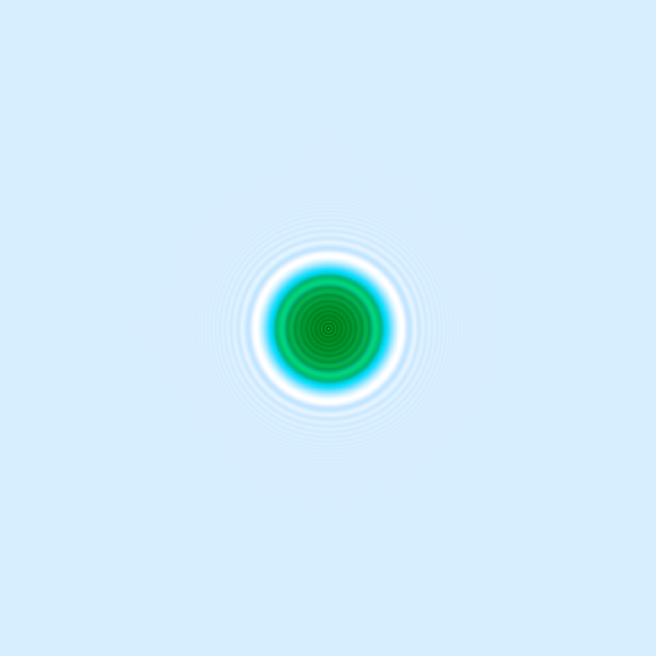
\includegraphics[width=\textwidth]{images/fig_sim_exitwave_multislice-r100-bd1e-3.png}}
		  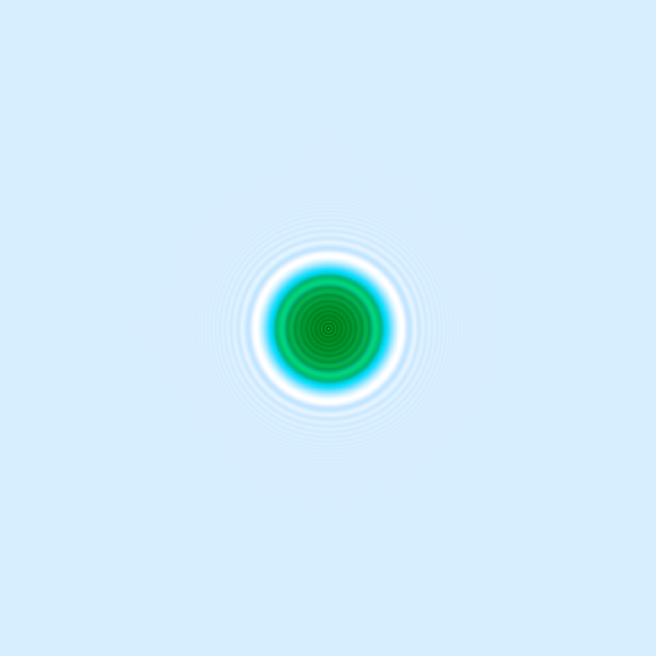
\includegraphics[width=\textwidth]{images/fig_sim_exitwave_multislice-r100-bd1e-3.png}\llap{\makebox[\wd1][l]{\includegraphics[width=0.5\textwidth]{images/fig_sim_exitwave_multislice_cw-r100-bd1e-3.pdf}}}
		  
		\caption{Austrittswelle}
		\label{fig:exitwave}
	\end{subfigure}
	\begin{subfigure}[b]{0.49\textwidth}
		 \setbox1=\hbox{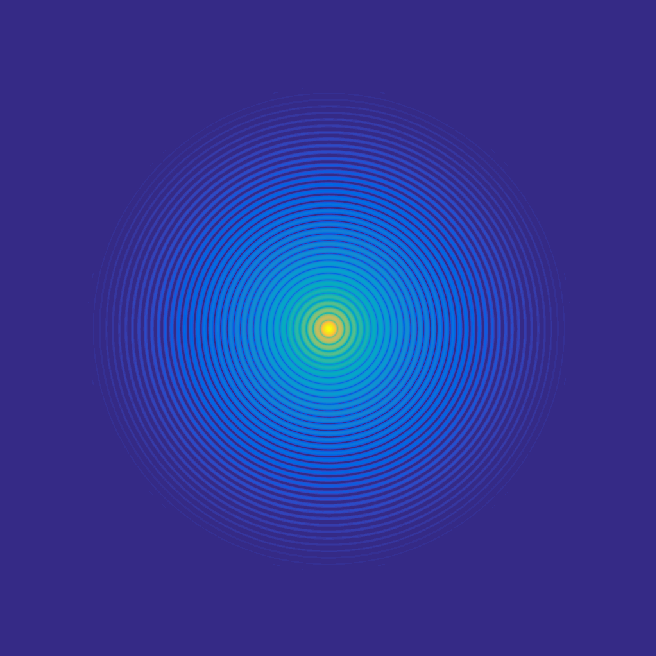
\includegraphics[width=\textwidth]{images/fig_sim_scatter_multislice-r100-bd1e-3.png}}
	 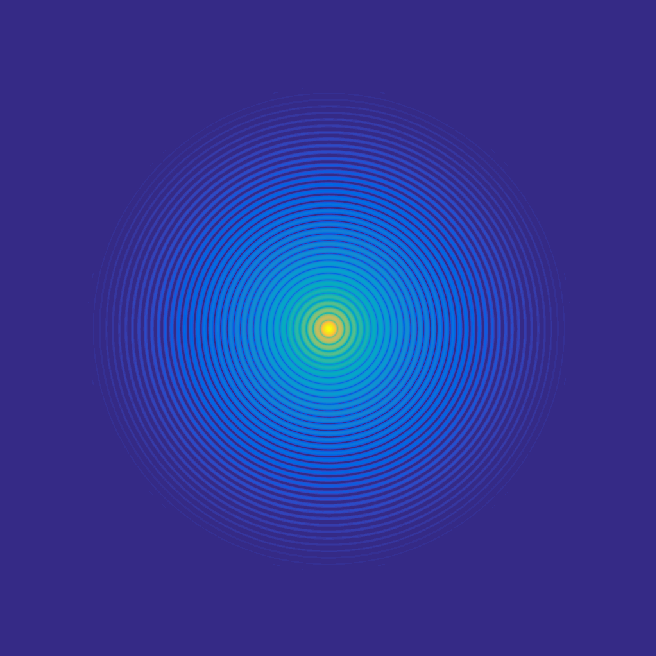
\includegraphics[width=\textwidth]{images/fig_sim_scatter_multislice-r100-bd1e-3.png}\llap{\makebox[\wd1][l]{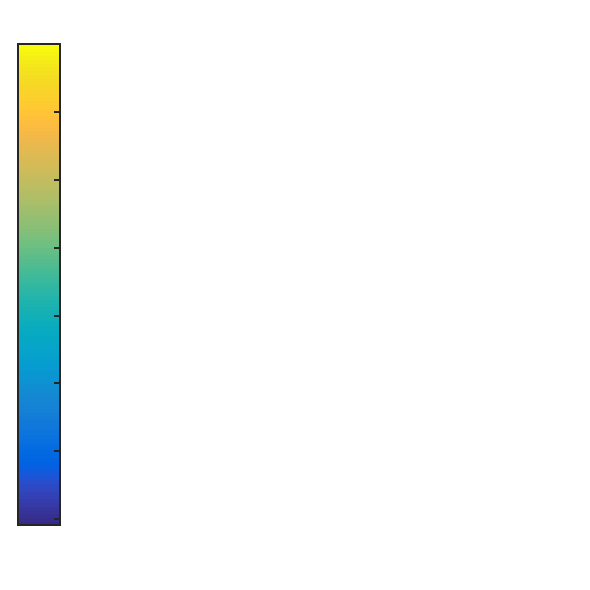
\includegraphics[width=0.5\textwidth]{images/fig_sim_scatter_multislice_cb-r100-bd1e-3.pdf}}}
		\caption{Streubild}
		\label{fig:scatter}
	\end{subfigure}
	\caption[Austrittswelle und Streubild einer Kugel]{Exemplarische Multislice-Propagations Austrittwelle und (logarithmiertes) Streubild einer Kugel mit Radius 100\si{nm} bei $\beta,\delta$=$10^{-3}$. Die relative Intensität der Austrittswelle bezüglich der Eintrittswelle ist über die Helligkeit dargestellt, die Phase über den Farbton. Das Streubild zeigt einen Bereich bis 15°.}
	\label{fig:exitscatter}
\end{figure}


\begin{figure}
	\centering
	\begin{subfigure}[b]{0.49\textwidth}
		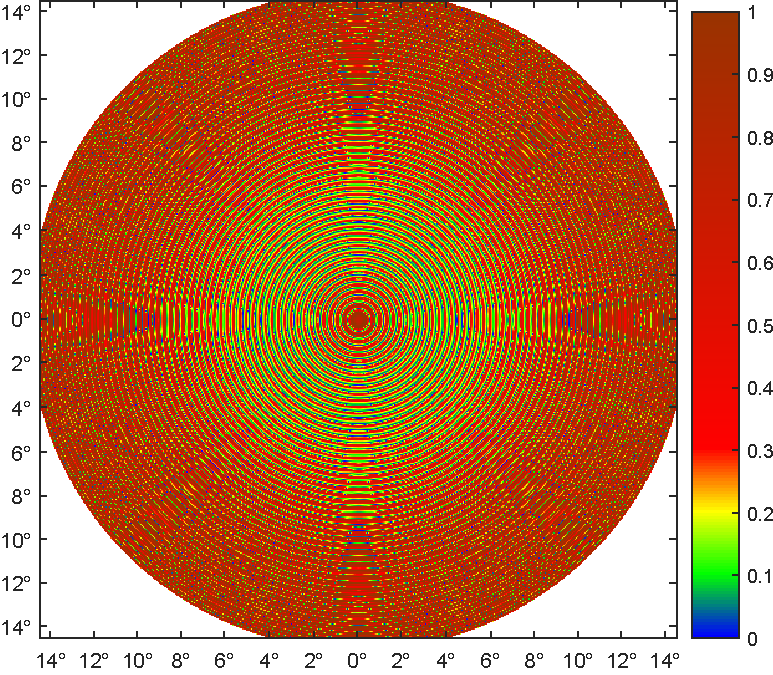
\includegraphics[width=\textwidth]{images/fig_sim_relerror_FTproj-r100-bd1e-3.pdf}
		\caption{Projektion}
	\end{subfigure}
	\begin{subfigure}[b]{0.49\textwidth}
		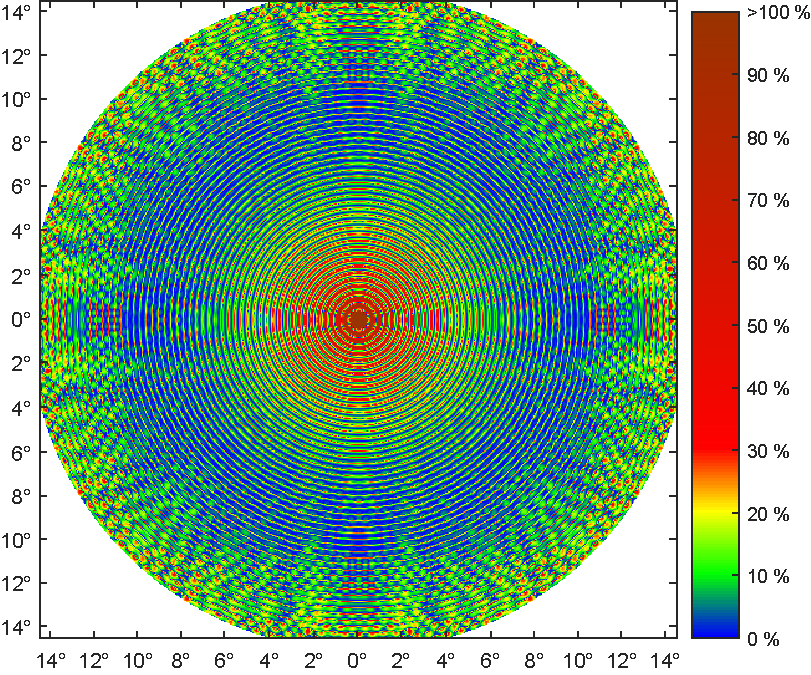
\includegraphics[width=\textwidth]{images/fig_sim_relerror_msft-r100-bd1e-3.pdf}
		\caption{MSFT}
	\end{subfigure}
	\\
	\begin{subfigure}[b]{0.49\textwidth}
		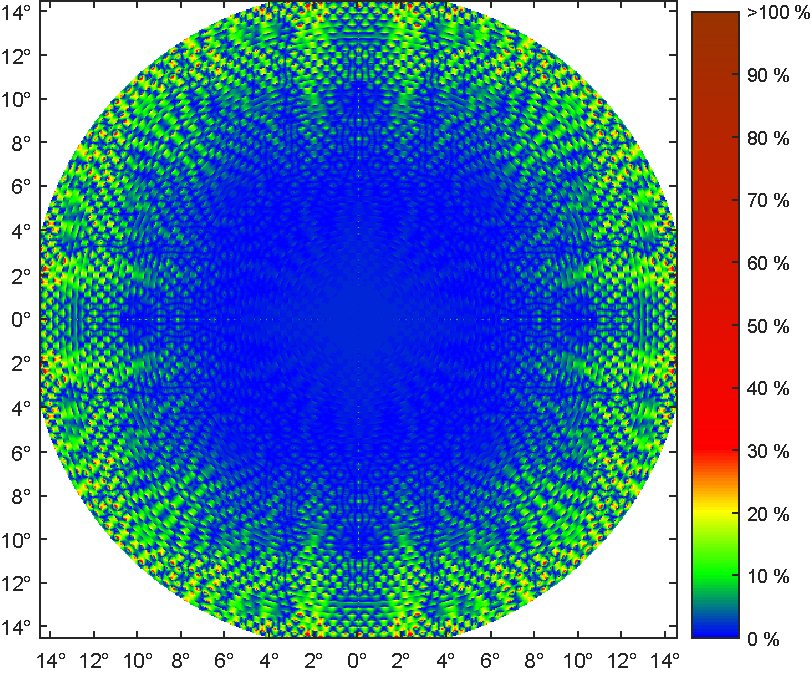
\includegraphics[width=\textwidth]{images/fig_sim_relerror_thibault-r100-bd1e-3.pdf}
		\caption{Thibaults Multislice}
	\end{subfigure}
	\begin{subfigure}[b]{0.49\textwidth}
		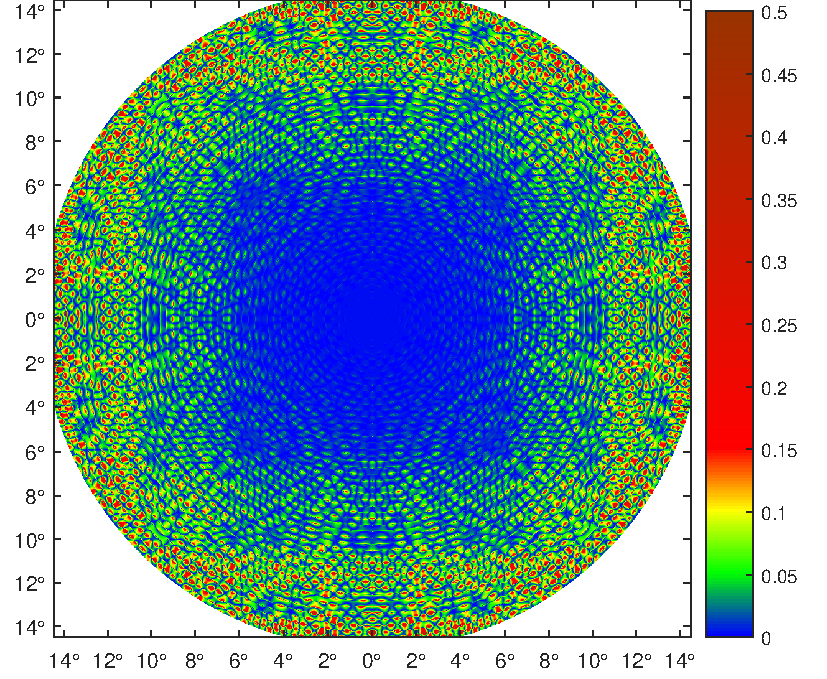
\includegraphics[width=\textwidth]{images/fig_sim_relerror_multislice-r100-bd1e-3.pdf}
		\caption{Multislice Propagation}
	\end{subfigure}
	
	\caption[relativer Fehler der Simulationen]{Relative Abweichungen von Mie der simulierten Streubilder einer Kugel mit Radius 100\si{nm} bei $\beta=\delta=10^{-3}$. }
	\label{fig:var}
\end{figure}


\begin{figure}
	\centering
	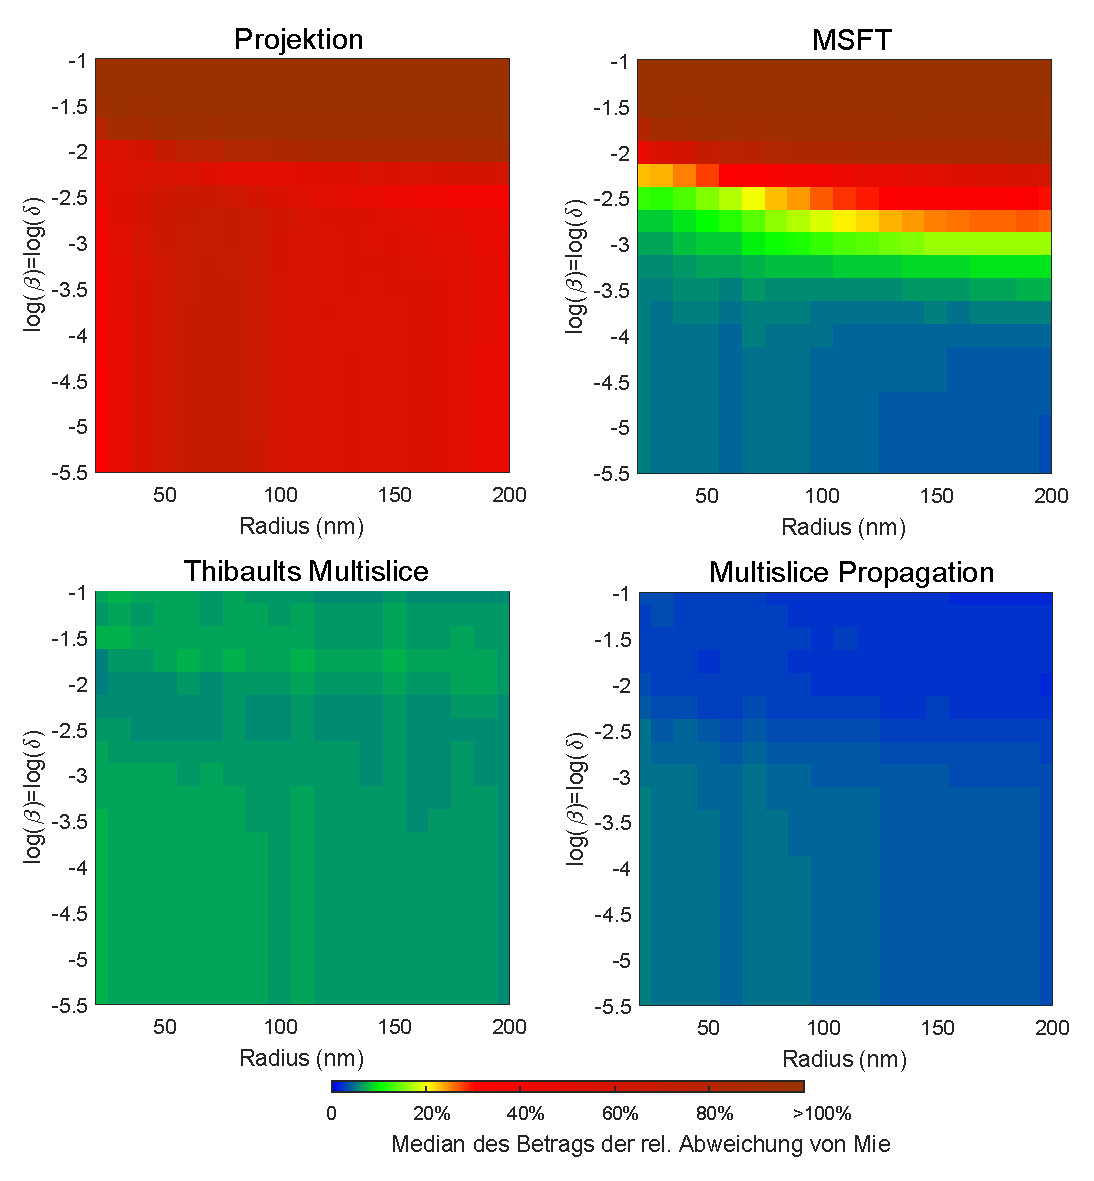
\includegraphics[width=1\textwidth]{images/fig_sim_var.pdf}
	\caption[Gültigkeit der Simulationsalgorithmen]{Zur Entscheidung bei welchen Radien und welchen Abweichung der Brechzahl vom Vakuum die Simulationen noch valide sind, ist die mediane, relative Abweichung von Mie über den Parametern aufgetragen. Es ist zu erkennen XXX}
	\label{fig:variation}
\end{figure}



\section{komplexe Objekte}
Neben der Berechnung von Streubilder von Kugeln eignen sich die Simulationsalgorithmen auch zur Berechnung der Austrittswellen und Streubilder hinter anderen Objekten.

Als interessante Testszene wird ein Ikosaeder mit eingebetteter Kugel sowie ein davon disjunktes, kleineres Dodekaeder betrachtet (Abb.)


